%% Overleaf			
%% Software Manual and Technical Document Template	
%% 									
%% This provides an example of a software manual created in Overleaf.

\documentclass[a4paper]{manual}

% Packages used in this example
\usepackage{graphicx}  % for including images
\usepackage{microtype} % for typographical enhancements
\usepackage{wrapfig} % for typographical enhancements
\usepackage{minted}    % for code listings
\usepackage{amsmath}   % for equations and mathematics
\setminted{style=friendly,fontsize=\small}
\usepackage{hyperref}  % for hyperlinks
\usepackage[a4paper,top=4.2cm,bottom=4.2cm,left=3.5cm,right=3.5cm]{geometry} % for setting page size and margins

% Custom macros used in this example document
\newcommand{\doclink}[2]{\href{#1}{#2}\footnote{\url{#1}}}
\newcommand{\cs}[1]{\texttt{\textbackslash #1}}

% Frontmatter data; appears on title page
\title{User Manual}

\version{0.2}
\author{Qian Qian}
\softwarelogo{\includegraphics[width=8cm]{pics/logo.png}}

\begin{document}

\maketitle

\tableofcontents
\newpage

\section{Introduction}
CoPilot serves as your driving companion. It is a \textbf{dashcam} which records your driving scene in high resolution. 

Moreover, different than any dashcam on the market, CoPilot has also \textbf{traffic light alert} system built in. It alerts the driver about the current traffic light status, using cutting-edge machine learning technology. 

One more thing, when parked, a \textbf{surveillance mode} can be activated, it will record the scene if motion is detected in the camera view. This gives your car another safety guard when parked in public, and collect evidence for hit-and-run incidence.

\section{Hardware Overview}
CoPilot consists of a 8MP front facing camera as its main sensor, in the enclosure it contains a Raspberrypi 3 and a real time clock. Two speakers are located on the sides for mode indication and voice alerts.
\begin{figure}[h!]
  \centering
  \includegraphics[width=.7\textwidth]{pics/front.jpg}
  \caption[]{CoPilot front.}
  \label{fig:front}
\end{figure}

On the back is a machine learning hardware accelerator for fast inference, and a Mode Selection button for switching between different modes. 
A small button for muting the voice alert is also available.
\begin{figure}[h!]
  \centering
  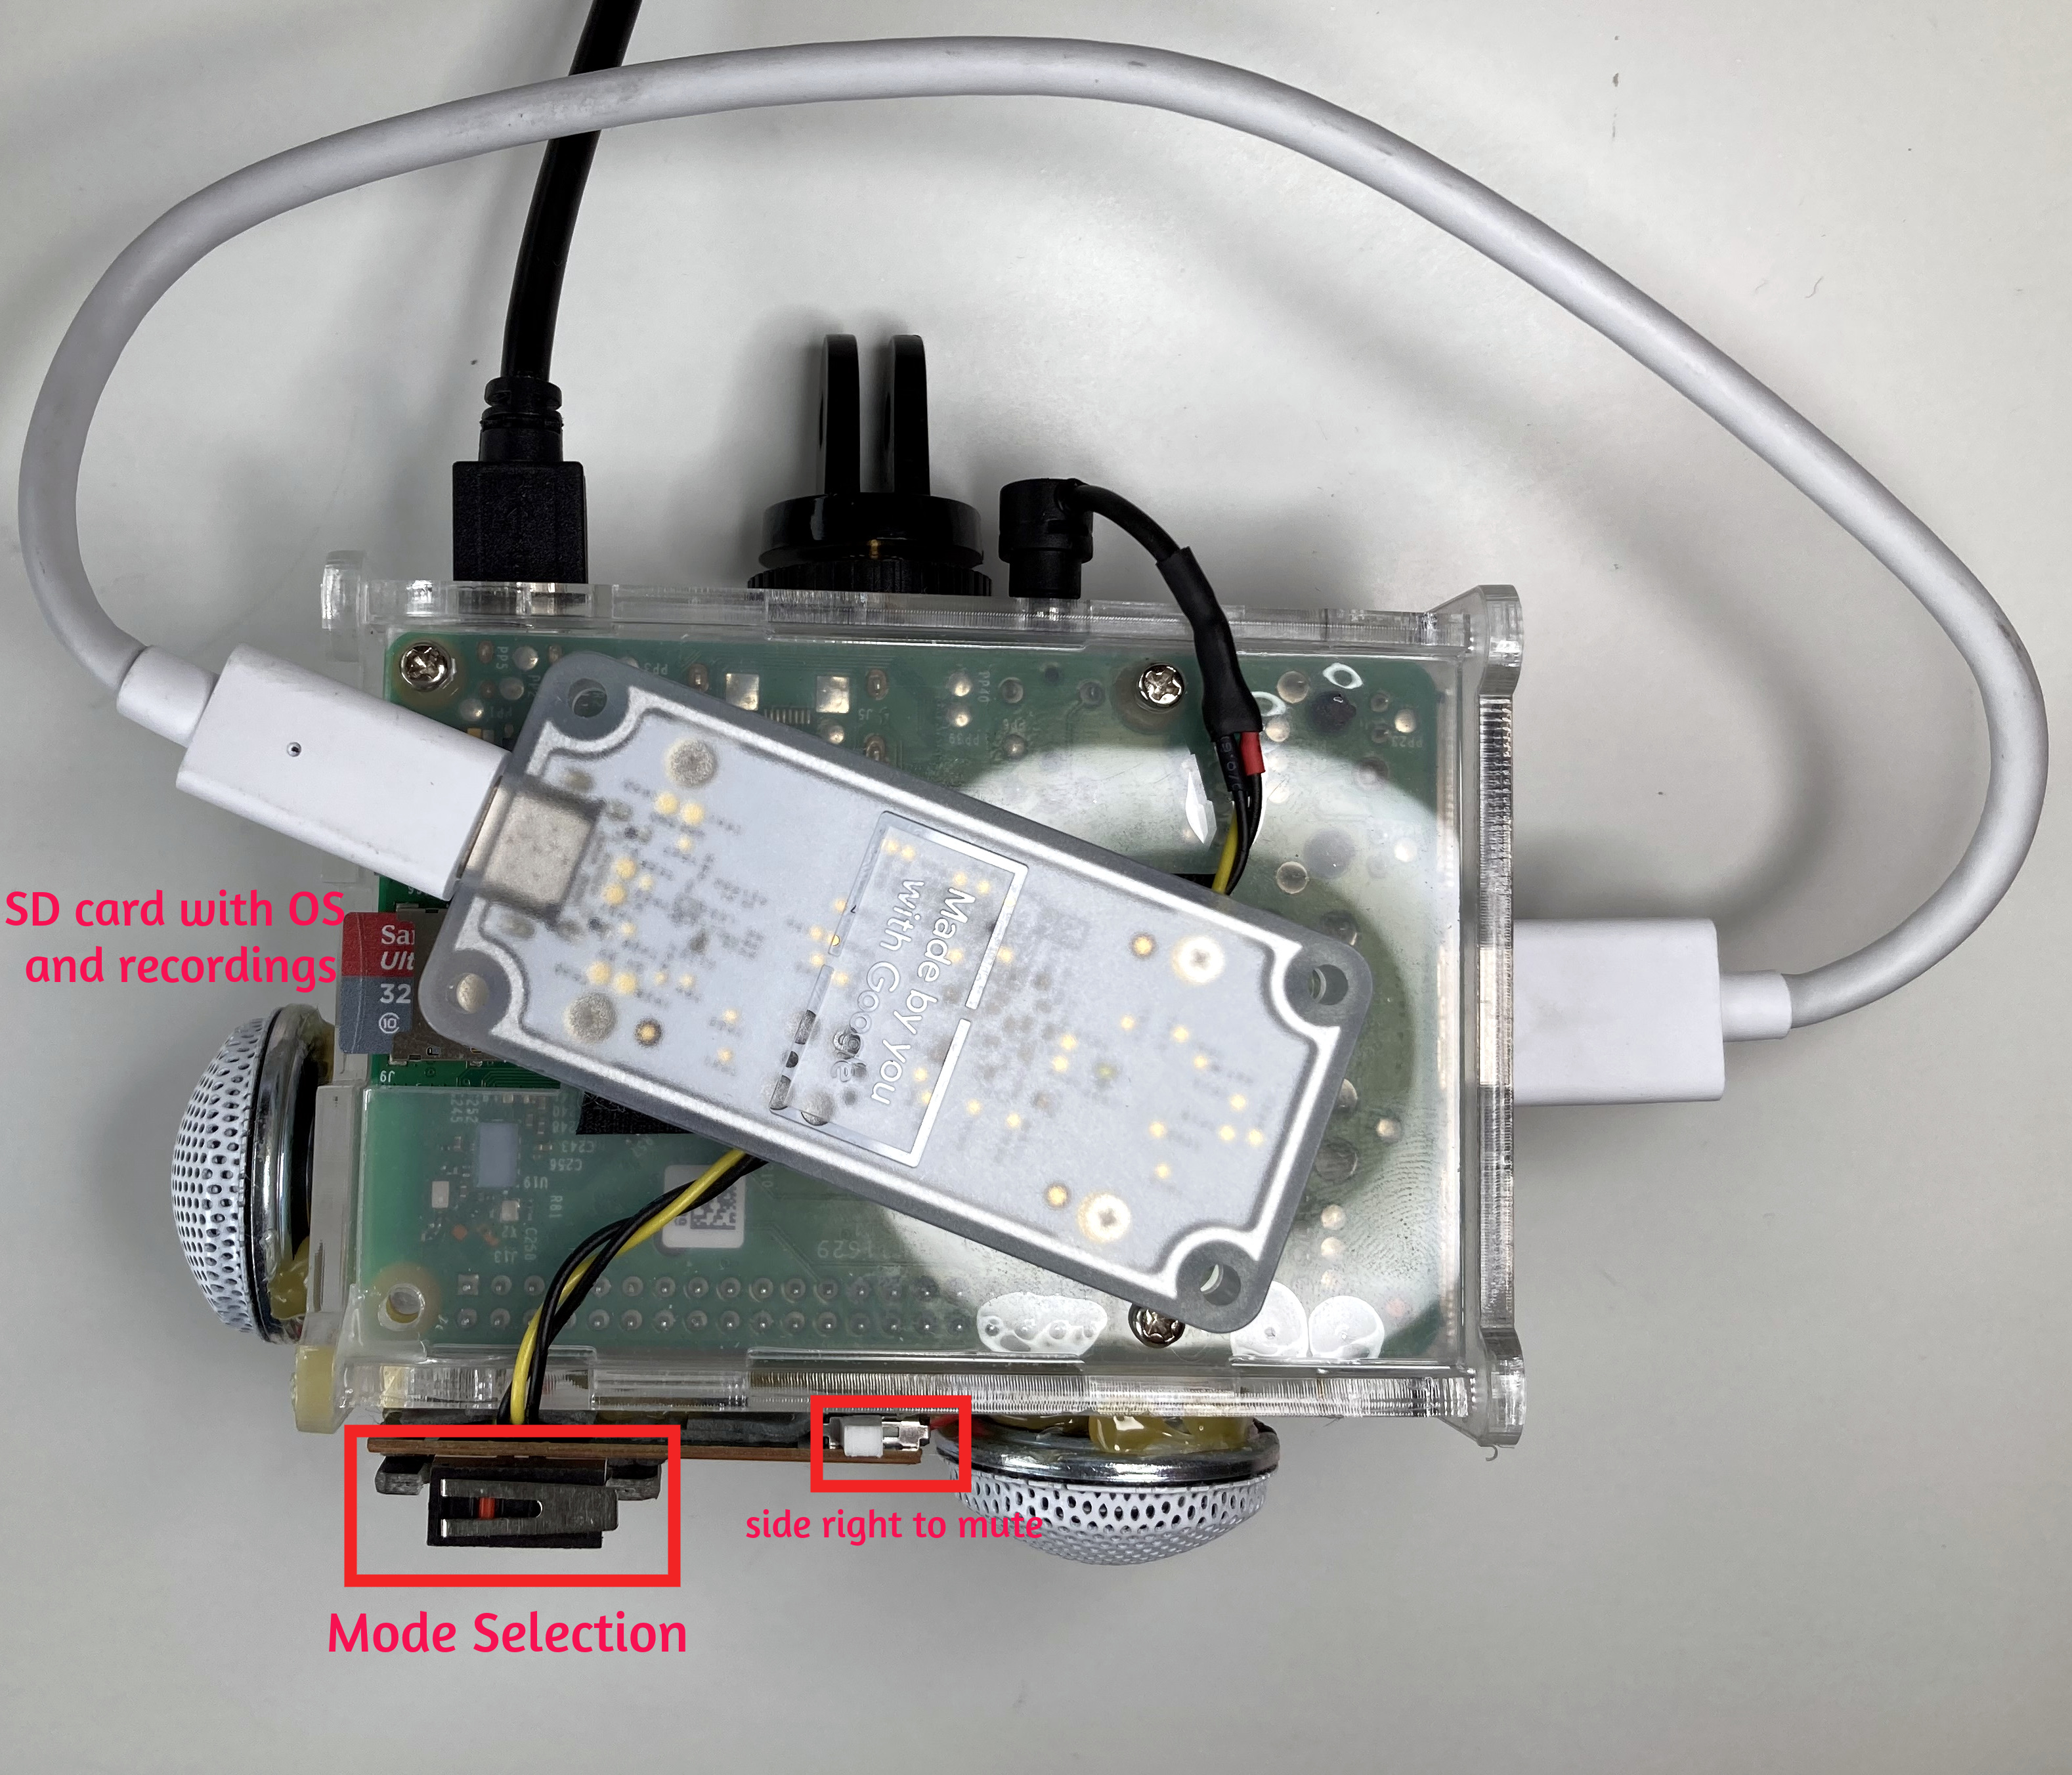
\includegraphics[width=.7\textwidth]{pics/back.png}
  \caption[]{CoPilot back.}
  \label{fig:front}
\end{figure}

\section{Installation Guide}
It is recommended to mount CoPilot in the \textbf{middle} of the windshield. \textbf{As high as possible} to have a better field of view. Adjust the angle of camera so that it is \textbf{facing straight forward}.
An example of mounting position is shown below:

\begin{figure}[h!]
  \centering
  \includegraphics[width=.65\textwidth]{pics/interior}
  \caption[]{Mounting position.}
  \label{fig:front}
\end{figure}

\section{Mode Selection}


\begin{table}[h!]
\centering
\caption{\label{tab:mode}Mode Selection.}
\begin{tabular}{l|c|c}
\hline
    Mode & Indicated Sound & Model Section Button\\\hline
    \textbf{Basic Alert Mode (Default)}& \emph{"Visibility Clear"} & Press once \\\hline
    \textbf{Experiment Alert Mode} & \emph{"Speed to Full"} & Press twice \\\hline
    \textbf{Surveillance Mode} & \emph{"Standing By"} & Press three times \\\hline
    \textbf{Error Mode} & \emph{"I am gone"} & Contact technical support \\\hline
\end{tabular}
\end{table}

\newcommand{\centered}[1]{\begin{tabular}{l} #1 \end{tabular}}

\subsection{Basic Alert Mode (Default)}
A subset of functionalities of the traffic light alert system will be activated.
\begin{table}[ht]
\caption{Basic alerts.}
\centering
\begin{tabular}{c|c}
\hline
    Scenario & Voice Alert \\
\hline
    \includegraphics[height=0.15\textwidth]{pics/red_to_green.png} &  "\emph{Ready go"/"Green go go go"}  \\
\hline
     \includegraphics[height=0.15\textwidth]{pics/green_to_yellow.png} &  "\emph{Yellow no rush"} \\
\hline
\end{tabular}
\label{tab:gt}
\end{table}

\clearpage
\subsection{Experiment Alert Mode}
Full functionalities of the traffic light alert system will be activated. It includes all the alerts from Basic Alert Mode, but also has more alerts shown below, where as soon as CoPilot
sees the first appearance of a traffic light it will alert its state.

\textbf{Note that due to the early stage of development, the false positive alert can significantly increase. Consequently it might disturb the driver while driving. Therefore this mode is not the default mode.}

\begin{table}[ht]
\caption{Additional alerts}
\centering
\begin{tabular}{c|c}
\hline
    Scenario & Voice Alert \\
\hline
    \includegraphics[height=0.15\textwidth]{pics/green.png} & \begin{tabular}{c} \emph{"Green go go go"} \end{tabular} \\
\hline
     \includegraphics[height=0.15\textwidth]{pics/red.png} & \begin{tabular}{c} \emph{"Attention Red"}\end{tabular} \\
\hline
\end{tabular}
\label{tab:gt}
\end{table}

\subsection{Surveillance Mode}

\begin{wrapfigure}{l}{4.5cm}
%\begin{figure}[h!]
  \includegraphics[width=.3\textwidth]{pics/motion_detection.jpg}
%\end{figure}
\end{wrapfigure}
Suitable for parked scenario, no traffic light alert in this mode. 

A recording of the scene will be created only when motion is detected.

\textbf{Note, in this mode, you might need to use an extenal power source like a power bank, since the in car USB power supply usually turns off when car is parked.} \\


\section{Recordings}
The recordings with be saved in the SD card shipped with CoPilot. New recordings will overwrite the old ones, if disk becomes full.
\textbf{Note the operating system is also located on the SD card. Deleting recordings is of course fine but please do not format the whole disk}. 



\end{document}
